\vspace*{2cm}
\thispagestyle{plain}

\begin{center}
    \phantomsection
    \addcontentsline{toc}{section}{Reading notes}

    \section*{\hfil Reading notes \hfil}
    \begin{justify}
        The links to the LaTeX source code and the latest version of this document can be found at \url{https://abishov.com/thesis/}. The implementation, documentation, and visualization demo can be found at \url{https://abishov.com/pvec-rs}.

        If you notice any typos while reading the document, or have any feedback in general, feel free to open an issue at \url{https://github.com/arazabishov/thesis/issues} or send me an email at \href{mailto:araz@abishov.com}{\nolinkurl{araz@abishov.com}}.
    \end{justify}

    \subsection*{\hfil Typographic conventions \hfil}
    \begin{tabular}{ r l }
        Clickable link & \href{https://www.rust-lang.org/}{Rust Programming Language} \\
        Inline code and types & \mintinline{rust}{Vec::new()} \\
        Project or library name & \emph{pvec-rs} \\
    \end{tabular}

    \vspace*{1cm}
    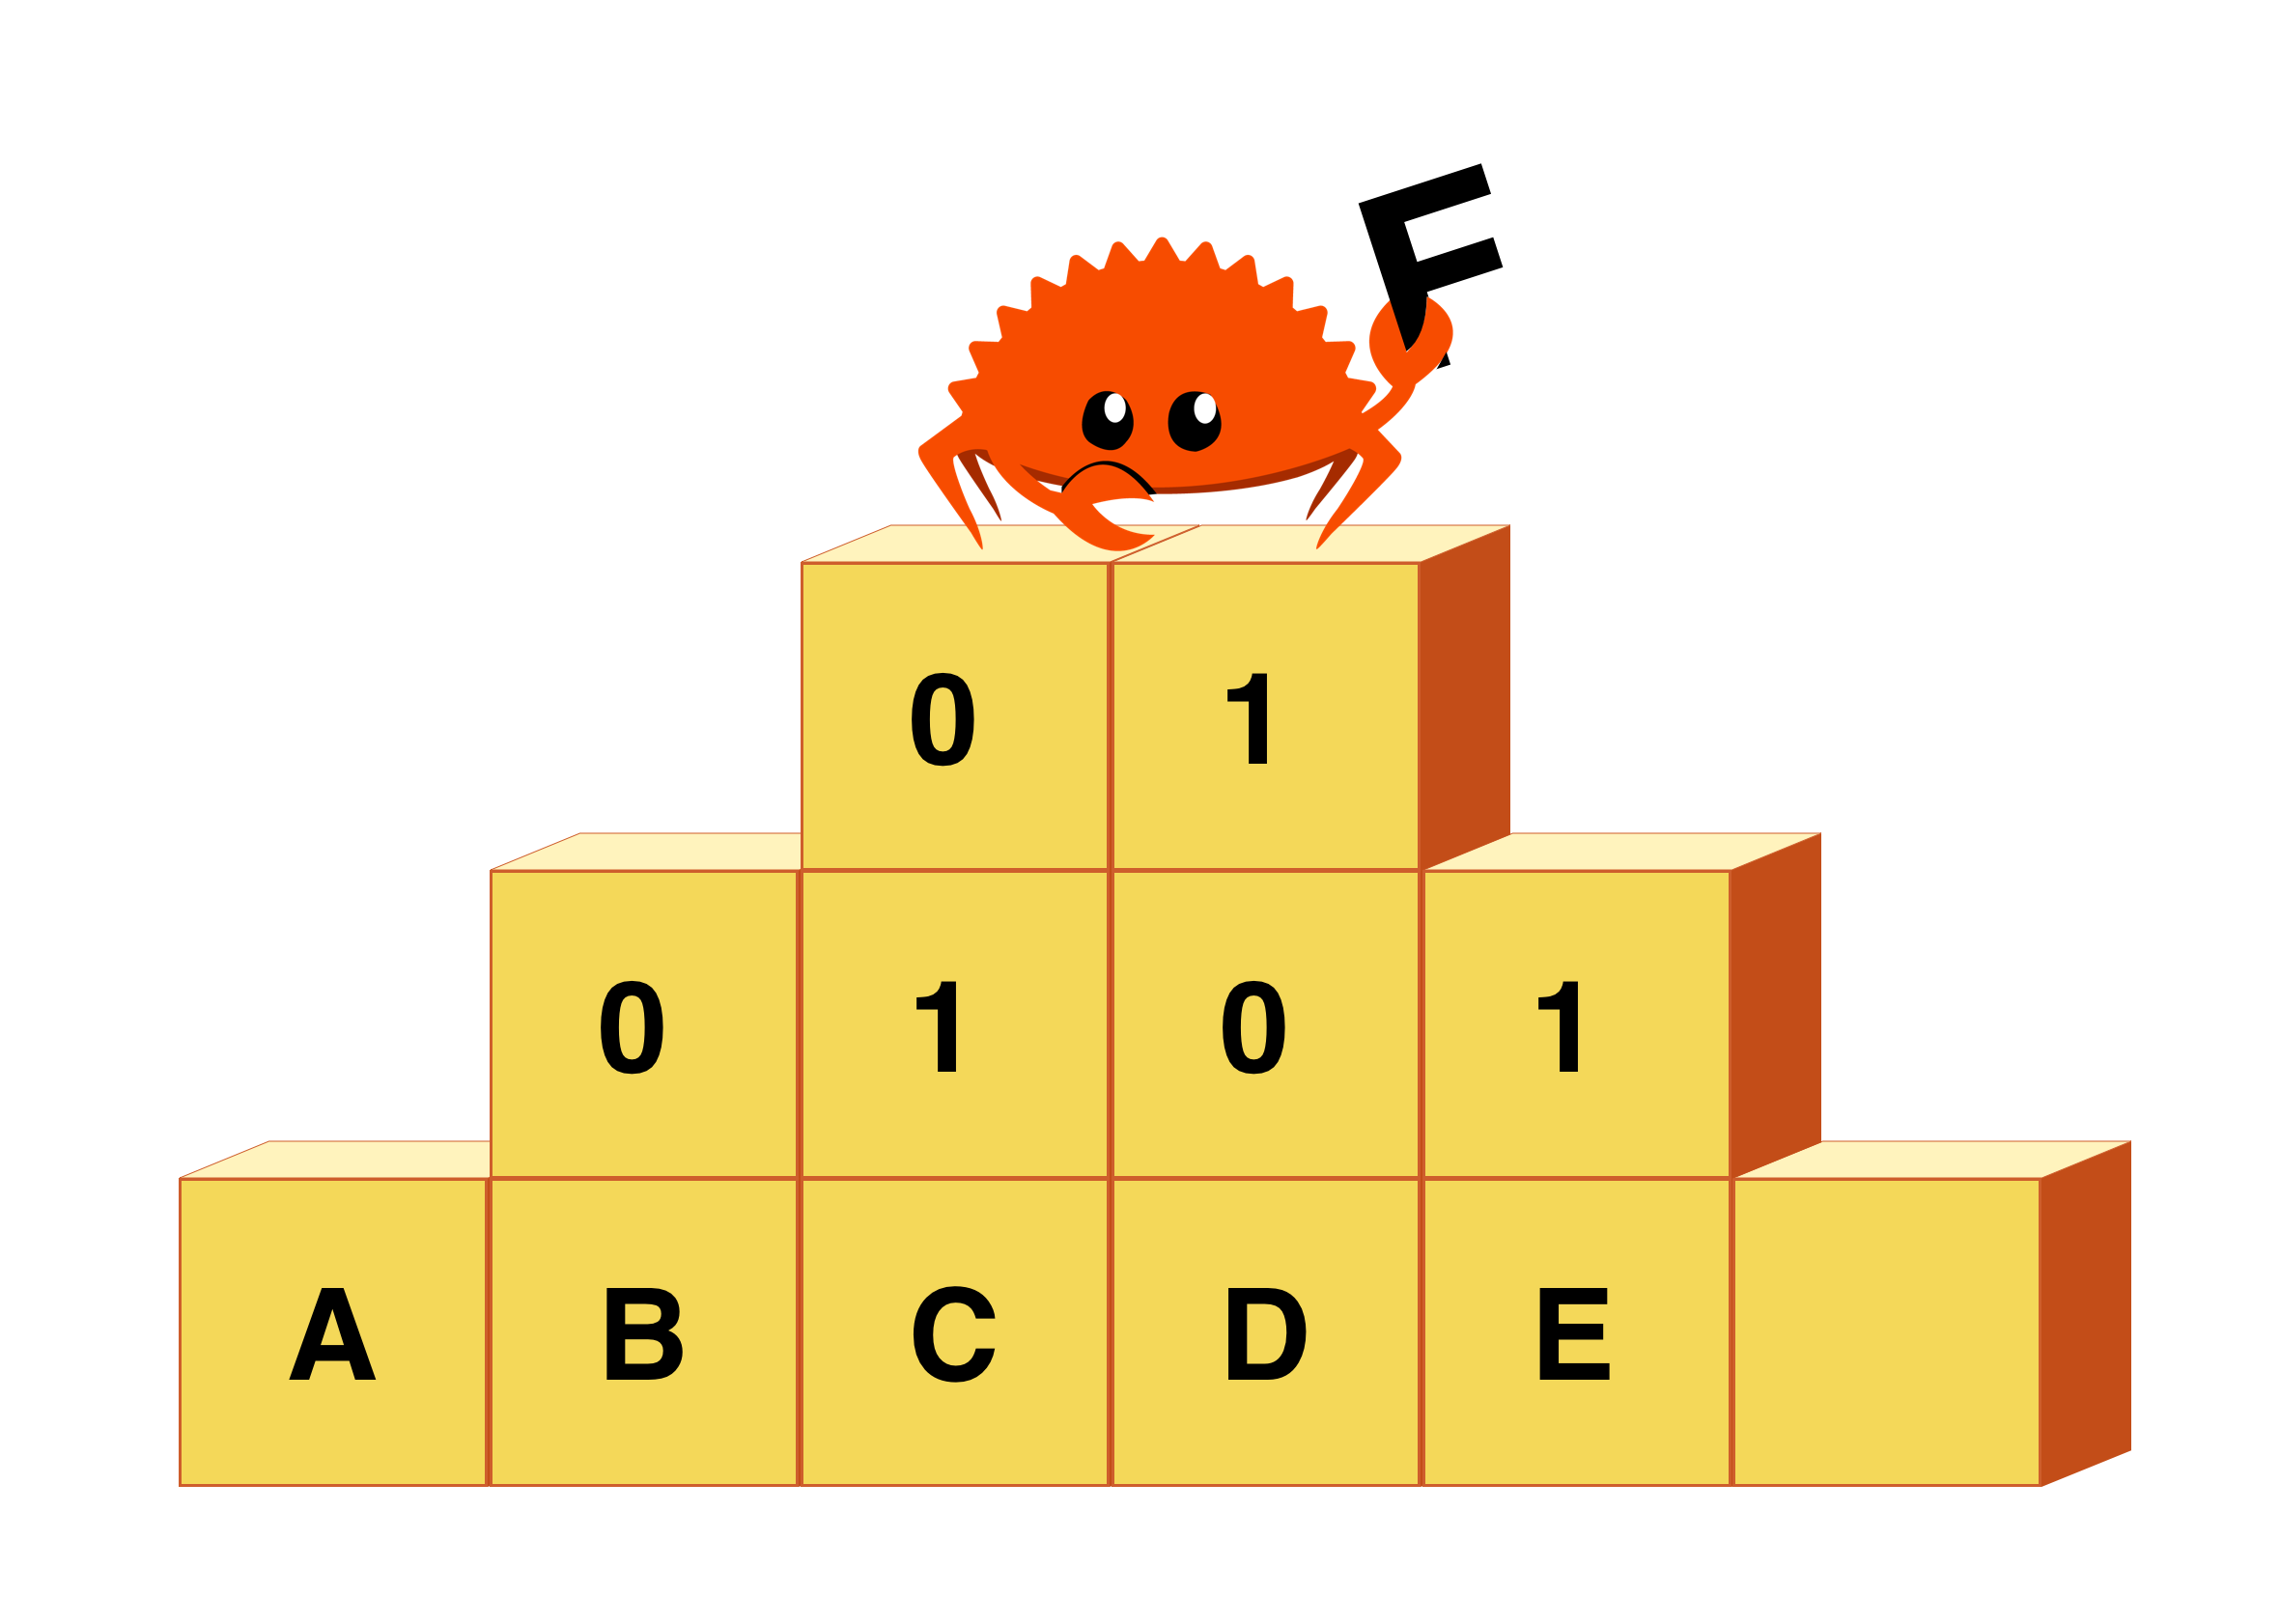
\includegraphics[width=8cm, angle=0, trim=10 10 10 10, clip]{images/ferris-climbing.png}
\end{center}

% TODO: explain the difference between \rrbtree{} and \treerrb{}, and how to interpret them.
% TODO: in general, you should define a consistent way to refer to concrete types and abstract concepts.
